\chapter{Anwendungen}
Um den Aufwand für die spätere Benutzung zu reduzieren ist zuerst eine allgemeine Implementation des \textsc{ESN}s geschrieben worden. 

\section{Vorhersage eines Rössler-Systems}
Eine erste Anwendung um die Möglichkeiten eines \textsc{ESN} zu demonstrieren besteht in der Vorhersage des Verhaltens eines \textit{Rössler-Systems}
\begin{align}
\label{eq:application_roessler_pde}
\begin{split}
\dot{x} &= -(y+z)\\
\dot{y} &= x + 0.25 \cdot  y\\
\dot{z} &= 0.4 + (x - 8.5)\cdot z.
\end{split} 
\end{align}

Hierbei werden zwei verschiedene Aufgaben betrachtet: (a) die Vorhersage von $x(n+50)$ durch die Kenntnis von $x(n)$ und (b) die Kreuz-Vorhersage $y(n)$ durch $x(n)$. Für beide Aufgaben wurde das System für jeweils $10000$ Schritte mit einer Abtastrate $\Delta t = 0.05$ simuliert, wobei die Hälfte der Daten für das Training und der Rest für die Testergebnisse verwendet worden ist.

\subsection{Vorhersage $x(n) \rightarrow x(n+48)$}
Hierfür ist durch eine \textsc{GridSearch} ein geeignetes System gefunden werden, Parameter in der Tabelle \ref{tab:application_roessler_a} dargestellt sind. Als Maß für die Optimierung wurde der \textit{Mean Square Error (MSE)} benutzt. 

\begin{table}[H]
	\centering
		\begin{tabular}{|c|c|}
		\rule[-1ex]{0pt}{4.5ex} Variable & \hspace{4ex} Wert \rule[-1ex]{4ex}{0pt}\\ 
		\hline \hline 
		\rule[-1ex]{0pt}{4.5ex} $N$ & $300$ \\ 
		\hline 
		\rule[-1ex]{0pt}{4.5ex} $\alpha$ & $0.10$ \\ 
		\hline 
		\rule[-1ex]{0pt}{4.5ex} $\rho$ & $0.035$ \\ 
		\hline 
	\end{tabular} 
	\caption{Auflistung der für (a) benutzten Parameter des \textsc{ESN}.}
\label{tab:application_roessler_a}
\end{table}
\begin{figure}[H]
    \centering
    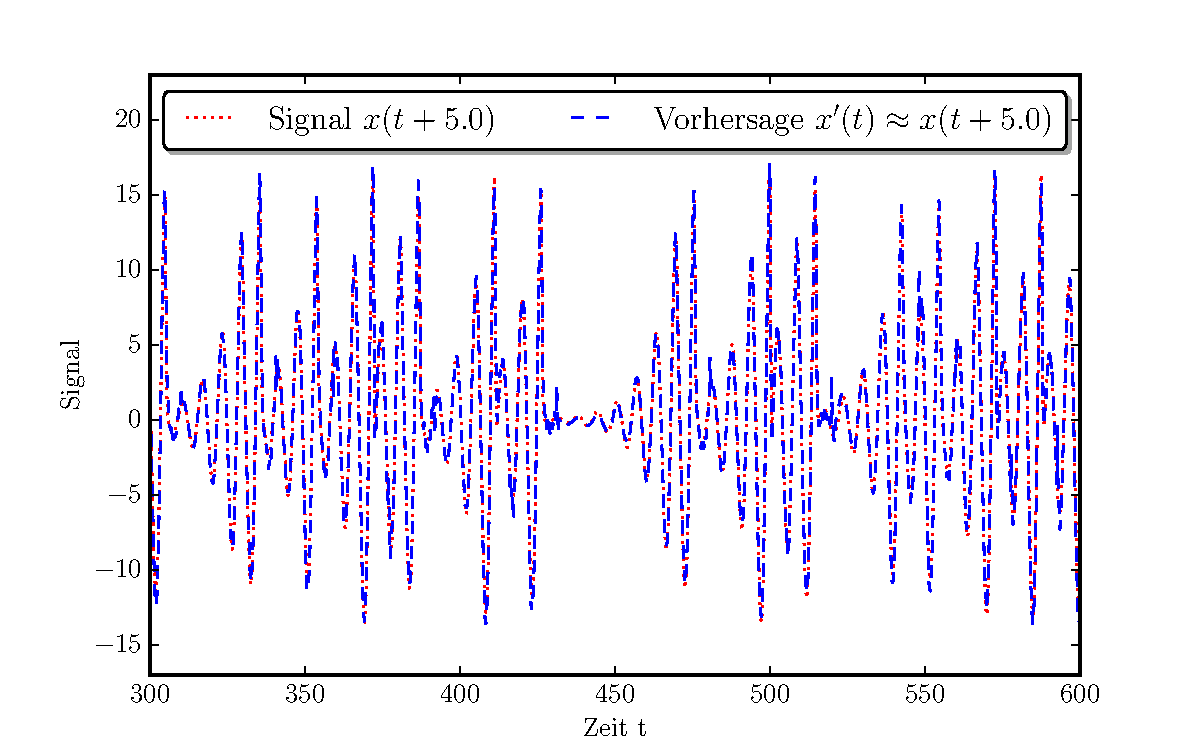
\includegraphics[width = 0.9 \textwidth]{figures/roessler_pred50.pdf}
    \caption{Graphische Darstellung des Signals $y(n)$ und der Vorhersage $y(n+50)$.}
    \label{fig:application_roessler_a}
\end{figure}

Hierbei wurde für den Trainingsvorgang ein Fehler $MSE = 0.575$ und für den Testvorgang von $MSE = 0.270$ bestimmt. Die grafische Darstellung der Vorhersage $v(n)$ und des ermittelten Fehlers sind in Abbildung \ref{fig:application_roessler_a} zu finden.

\subsection{Kreuz-Vorhersage $x(n) \rightarrow y(n)$}
Auch hierfür konnte sehr schnell durch eine \textsc{GridSearch} ein geeignetes System gefunden werden. Als Maß wurde ebenfalls der \textit{MSE} benutzt. Die gefundenen Parameter sind in der Tabelle \ref{tab:application_roessler_b} dargestellt.

\begin{table}[H]
	\centering
		\begin{tabular}{|c|c|}
		\rule[-1ex]{0pt}{4.5ex} Variable & \hspace{4ex} Wert \rule[-1ex]{4ex}{0pt}\\ 
		\hline \hline 
		\rule[-1ex]{0pt}{4.5ex} $N$ & $500$ \\ 
		\hline 
		\rule[-1ex]{0pt}{4.5ex} $\alpha$ & $0.20$ \\ 
		\hline 
		\rule[-1ex]{0pt}{4.5ex} $\rho$ & $0.01$ \\ 
		\hline 
	\end{tabular} 
	\caption{Auflistung der für (b) benutzten Parameter des \textsc{ESN}.}
\label{tab:application_roessler_b}
\end{table}

Für das Auslesen wurde eine Linearkombination genutzt, für die die Lösung $\mathbf{W}_{out}$ mittels der Pseudoinversen bestimmt werden konnte.

\begin{figure}[H]
    \centering
     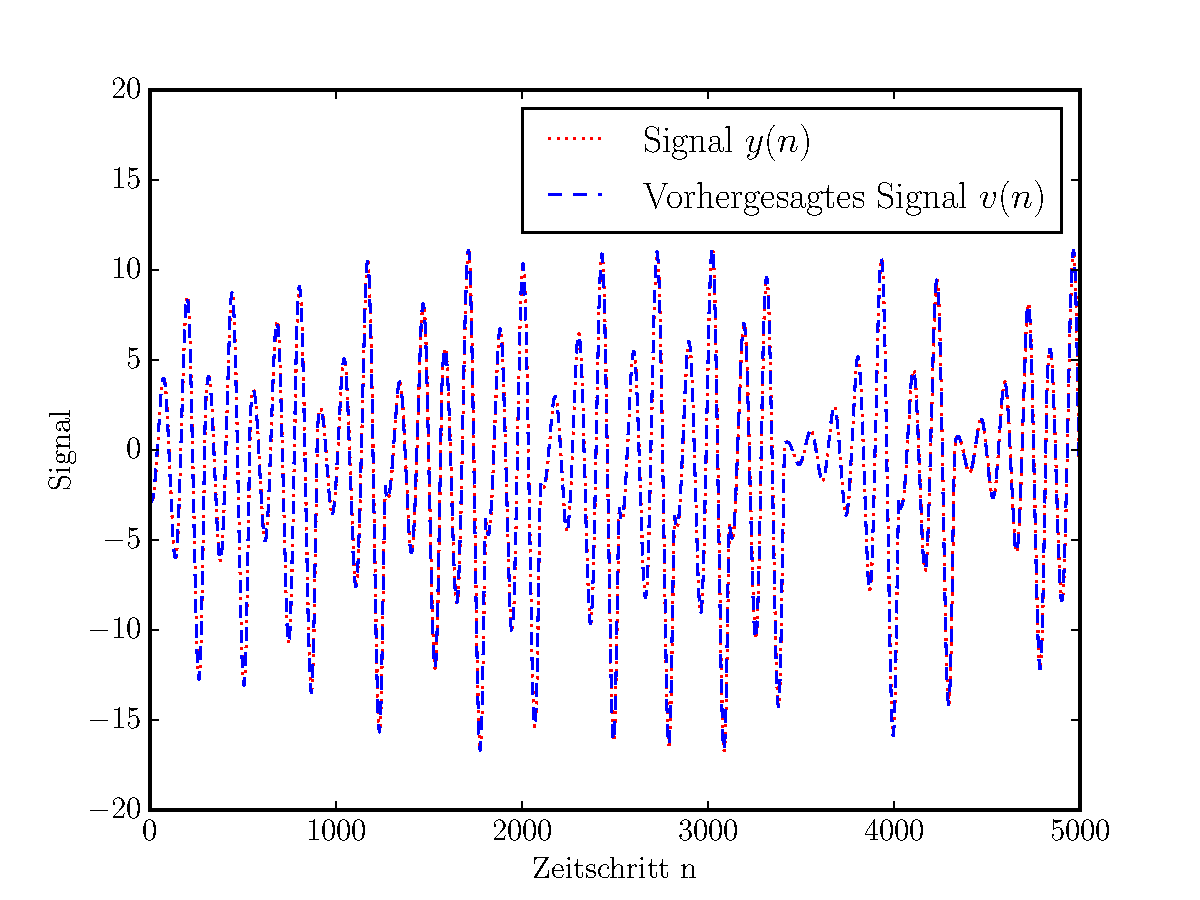
\includegraphics[width = 0.9 \textwidth]{figures/roessler_cross_pred.pdf}
    \caption{Graphische Darstellung des Signals $y(n)$ und der Vorhersage $v(n)$.}
    \label{fig:application_roessler_b1}
\end{figure}

Hierbei wurde für den Trainingsvorgang ein Fehler $MSE = 0.011$ und für den Testvorgang von $MSE = 0.091$ bestimmt. Die grafische Darstellung der Vorhersage $v(n)$ und des ermittelten Fehlers sind in Abbildungen \ref{fig:application_roessler_b1}, \ref{fig:application_roessler_b2} zu finden.

\begin{figure}[H]
    \centering
    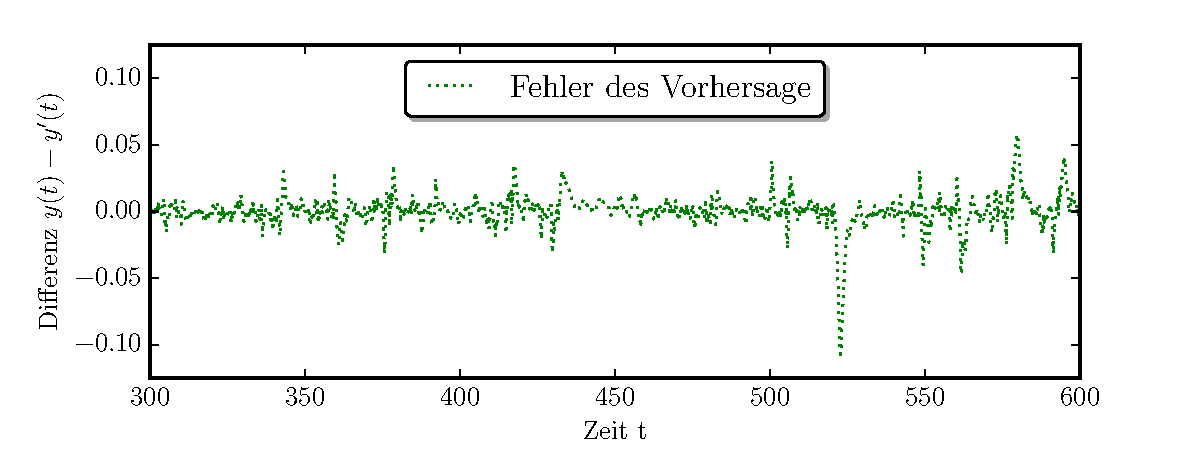
\includegraphics[width = 0.9 \textwidth]{figures/roessler_cross_err.pdf}
    \caption{Graphische Darstellung des des Fehlers $y(n)-v(n)$.}
    \label{fig:application_roessler_b2}
\end{figure}

\section{Vorhersage eines Mackey-Glass-Systems}
asdasd